%%%%%%%%%%%%%%%%%%%%%%%%%%%%%%%%%%%%%%
% Beamer Presentation
% LaTeX Template
% Version 1.0 (10/11/12)
%
% This template has been downloaded from:
% http://www.LaTeXTemplates.com
%
% License:
% CC BY-NC-SA 3.0 (http://creativecommons.org/licenses/by-nc-sa/3.0/)
%
%%%%%%%%%%%%%%%%%%%%%%%%%%%%%%%%%%%%%%%%%

%----------------------------------------------------------------------------------------
%	PACKAGES AND THEMES
%----------------------------------------------------------------------------------------

\documentclass{beamer}

\mode<presentation> {

% The Beamer class comes with a number of default slide themes
% which change the colors and layouts of slides. Below this is a list
% of all the themes, uncomment each in turn to see what they look like.

% \usetheme{default}
% \usetheme{AnnArbor}
% \usetheme{Antibes}
% \usetheme{Bergen}
% \usetheme{Berkeley}
% \usetheme{Berlin} #
% \usetheme{Boadilla}
% \usetheme{CambridgeUS}
% \usetheme{Copenhagen}
% \usetheme{Darmstadt}
% \usetheme{Dresden}
% \usetheme{Frankfurt}
% \usetheme{Goettingen}
% \usetheme{Hannover}
% \usetheme{Ilmenau}
% \usetheme{JuanLesPins}
% \usetheme{Luebeck}
% \usetheme{Madrid}
% \usetheme{Malmoe}
% \usetheme{Marburg}
% \usetheme{Montpellier}
% \usetheme{PaloAlto}
% \usetheme{Pittsburgh}
\usetheme{Rochester}
% \usetheme{Singapore}
% \usetheme{Szeged}
% \usetheme{Warsaw}

% As well as themes, the Beamer class has a number of color themes
% for any slide theme. Uncomment each of these in turn to see how it
% changes the colors of your current slide theme.

% \usecolortheme{albatross}
% \usecolortheme{beaver}
% \usecolortheme{beetle}
% \usecolortheme{crane}
\usecolortheme{dolphin}
% \usecolortheme{dove}
% \usecolortheme{fly}
% \usecolortheme{lily}
% \usecolortheme{orchid}
% \usecolortheme{rose}
% \usecolortheme{seagull}
% \usecolortheme{seahorse}
% \usecolortheme{whale}
% \usecolortheme{wolverine}

%\setbeamertemplate{footline} % To remove the footer line in all slides uncomment this line
%\setbeamertemplate{footline}[page number] % To replace the footer line in all slides with a simple slide count uncomment this line

\setbeamertemplate{navigation symbols}{} % To remove the navigation symbols from the bottom of all slides uncomment this line
}
\usepackage{amssymb}
\usepackage{mathtools}
\usepackage{undertilde}
\usepackage{amsmath}
\usepackage{graphicx} % Allows including images
\usepackage{booktabs} % Allows the use of \toprule, \midrule and \bottomrule in tables
\usepackage{threeparttable}

%----------------------------------------------------------------------------------------
%	TITLE PAGE
%----------------------------------------------------------------------------------------

\title[Scotch Recommender]{An NLP-Based Scotch Whisky Recommender Agent} % The short title appears at the bottom of every slide, the full title is only on the title page

\author{Robert Soane} % Your name
\institute[14302983] % Your institution as it will appear on the bottom of every slide, may be shorthand to save space
{
14302983 \\ % Your institution for the title page
\medskip
}
\date{\today} % Date, can be changed to a custom date


\begin{document}

\begin{frame}
\titlepage % Print the title page as the first slide
\end{frame}

%----------------------------------------------------------------------------------------
%	PRESENTATION SLIDES
%----------------------------------------------------------------------------------------

%------------------------------------------------
\section{Scotch Whisky} 
%------------------------------------------------

\subsection{Brief Overview} % A subsection can be created just before a set of slides with a common theme to further break down your presentation into chunks

\begin{frame}
\frametitle{The Scotch Market}
The Scotch whisky industry is massive.
\begin{itemize}
    \item 75\% of Scotland's food and drink exports.
    \item Over 20\% of the UK's food and drink exports.\footnote{https://www.scotch-whisky.org.uk/insights/facts-figures/}
    \item Over 130 disilleries in Scotland.\footnote{https://whiskytastingcompany.com/blogs/news/how-many-whisky-distilleries-are-in-scotland}
\end{itemize}

\end{frame}

\begin{frame}
    \frametitle{Distillation}
    The approximate whisky production process:\footnote{K. Jacques, T. Lyons, and D. Kelsall, The Alcohol Textbook 4th edition, 4th ed. Nottingham
    University Press, 2003.}
    \begin{itemize}
        \item Grains germinate to develop sugars
        \item Sugars extracted to produce \emph{wort}
        \item Wort fermented
        \item Beer distilled
        \item \emph{New make} aged
    \end{itemize}

    \begin{block}{The Law}
        Legal definition of Scotch:\footnote{legislation.gov.uk/uksi/2009/2890/regulation/3/made}
        \begin{itemize}
            \item Aged in oak casks
            \item Minimum age = 3 years
            \item ABV $\geq$ 40\%
            \item Entire production process in Scotland
        \end{itemize}
        
    \end{block}
\end{frame}

\subsection{Whisky and Words}
\begin{frame}
    \frametitle{Single, Malt, Blends and Grain}
    \begin{itemize}
        \item `Single' $\implies$ One distillery.
        \item `Malt' $\implies$ 100\% malted barley
        \item `Blended' $\implies$ Multiple distilleries
        \item `Grain' $\implies$ Any grain, not just malt.
    \end{itemize}
    
\end{frame}

\begin{frame}
    \frametitle{Flavour Dimensions}
    Various whisky-specific words are used.\footnote{
        G. N. Bathgate, ``The influence of malt and wort processing on spirit character: the lost styles of
    Scotch malt whisky,'' \emph{Journal of the Institute of Brewing}, vol. 125, no. 2, pp. 200-213, 2019}
    \footnote{J. Mosedale and J.-L. Puech, ``Wood maturation of distilled beverages'', \emph{Trends in
    Food Science \& Technology}, vol. 9, no. 3, pp. 95-101, mar 1998. Available:
    https://linkinghub.elsevier.com/retrieve/pii/S0924224498000247}
    
    \begin{block}{Peat}
    Smoky flavour imparted on Scotch from peat fires used dry malt/grain.
    \end{block}

    \begin{block}{Sherry}
    Descriptor for flavours imparted on Scotch from aging in casks previously used to age sherry.
    \end{block}
\end{frame}

\subsection{Statement of Problem}

\begin{frame}{Statement of Problem}

    \textbf{This project sought to apply NLP techniques to produce a recommender agent and ascertain whether
    NLP techniques applied to Whisky tasting notes can power an effective recommender agent.}
\end{frame}

%------------------------------------------------
\section{Background and Literature} 
%------------------------------------------------

\subsection{NLP and Language Models}

\begin{frame}
    \frametitle{Mapping Text to a Vector Space}
    \begin{itemize}
        \item Need a model to transform text.
        \item Common models transform the text to a vector space.\footnote{https://ieeexplore.ieee.org/document/6786458}
        \item Root form transformations - stemming, lemmatization etc.
        \item Bag of Words \& Word2vec
    \end{itemize}
\end{frame}

\begin{frame}
    \frametitle{Keyword Extraction}
    \begin{itemize}
        \item To build BoW need keywords
        \item Various methods can be used
        \item TF-IDF
        \item Graph Based Methods\footnote{https://hrcak.srce.hr/140857}
    \end{itemize}
\end{frame}

\begin{frame}
    \frametitle{Graph Based KE}
    \begin{itemize}
        \item Co-occurence graph
        \item Each node represents a candidate keyword
        \item Centrality measures are used to select keywords
        \item RAKE\footnote{ S. Rose, D. Engel, N. Cramer, and W. Cowley, 
        ``Automatic keyword extraction,'' \emph{Text Mining:
        Applications and Theory}, pp. 1-277, 2010}, Eigencentrality\footnote{https://linkinghub.elsevier.com/retrieve/pii/S0378873307000342}
    \end{itemize}
    \begin{block}{Eigencentrality}
        Each node's centrality proportional to all adjacent nodes.
        \begin{itemize}
            \item Adjacency Graph $A$ 
            \item $i^{th}$ node's score $x_i$ 
            \item $x_i = \frac{1}{\lambda}A_{ij}x_j$
            \item $\textbf{A}\cdot \utilde{x} = \lambda \utilde{x}$
        \end{itemize}

    \end{block}
\end{frame}

\subsection{Recommender Agents}
\begin{frame}
    \frametitle{Recommender Agents}
    \begin{itemize}
        \item \textbf{Collaborative Filtering (CF): }Based on users habits.
        \item \textbf{Content Based (CB): }Based on details about instances in data set.
    \end{itemize}
\end{frame}

\subsection{AI Applications to Whisky}
\begin{frame}
    \frametitle{AI Applications to Whisky}
    \textbf{Large gap in the research}
    \begin{itemize}
        \item Small number of CF and CB agents have been produced.
        \item Predominantly based on distinct features, or the users
        entire profile.
    \end{itemize}
\end{frame}

\begin{frame}
    \frametitle{Classification of Single Malt Whiskies}
    One piece of research into clustering of Scotch using tasting note data:\footnote{https://link.springer.com/chapter/10.1007/978-3-642-59789-3\_14}
    \begin{itemize}
        \item Used tasting notes to cluster 80 whiskies
        \item Very much aimed at finding specific details of flavour dimensions
        \item Interesting research, working with industry
    \end{itemize}
    This project aims instead to produce an autonomous agent to recommend whiskies.
\end{frame}

%------------------------------------------------
\section{Approach and Implementation} 
%------------------------------------------------

\subsection{The Agent and the Environment}
\begin{frame}
    \frametitle{The Agent and the Environment}
    \begin{itemize}
        \item \textbf{The Agent:} Recommends based on user input and 
        tasting notes. Capacity to autonomously update database.
        \item \textbf{The Environment:} The user input, and an online spirits
        shop.
    \end{itemize}
\end{frame}

\subsection{The Data}
\begin{frame}
    \frametitle{Web Scraping}
    The dataset was scraped from the Master of Malt website using a python 
script.\footnote{http://masterofmalt.com/}

The agent update function scrapes the new additions to the website. 
IDs are created using an MD5 hash - the update function stops updating 
after it achieves a number of duplicates.

The model is re-trained after each update.
\end{frame}

\subsection{NLP Choices and Training}
\begin{frame}{KE and Lemmatizing}
\begin{columns}[c] % The "c" option specifies centered vertical alignment while the "t" option is used for top vertical alignment
\column{.45\textwidth} % Left column and width
\begin{itemize}
    \item The Scotch lexicon leads to poor lemmatization attempts
    \item WordNet $:$ `peated' $\rightarrow$ `peated'
    \item Whisky tasting notes are very feature rich
    \item Default lemmatizer and KE methods performed poorly
    \item Implemented an Eigencentrality KE method in Python
\end{itemize}
        
\column{.5\textwidth} % Right column and width
\begin{table}
    \centering
    \begin{threeparttable}

        \caption{Times of TF-IDF, RAKE and eRAKE with various lemmatizers in seconds.}\label{tab:times}
        \begin{tabular}{llll} 
        \toprule
                           & TF-IDF        & RAKE           & eRAKE           \\
        U       & \textit{1247} & \textit{0.441} & \textit{-}      \\
        WN & \textit{1461} & \textit{130.2} & \textit{-}      \\
        WL   & \textit{1209} & \textit{4.947} & \textit{47.6}  \\
        \bottomrule
        \end{tabular}
        \begin{tablenotes}
            \small
            \item \textbf{Note:} eRAKE was only applied to the WhiskyLemmatized corpus
            as the eRake implementation included the WhiskyLemmatizer.
            \item \emph{u}: Unlemmatized, \emph{WN}: WordNet, \emph{WL}: Whisky
        \end{tablenotes}
    \end{threeparttable}
\end{table}
\end{columns}
\end{frame}



\begin{frame}{Clustering}
    Implemented clustering for sanity check, and qualitative comparison
    of different KE methods.
    \begin{itemize}
        \item Found that RAKE performed poorly - unsurprising as RAKE is 
        aimed at features with higher relative frequency.  Unsuited to
        tasting notes.
        \item eRAKE and TF-IDF performed similarly.
    \end{itemize}
\end{frame}

\begin{frame}{Training Process}
    \begin{itemize}
        \item eRAKE method lemmatizes tasting notes and performs KE 
        \item Each whisky vectorised
        \item Dataset transformed to a matrix
        \item Model created for each of \emph{nose}, \emph{palate}, \emph{finish} and \emph{general}
    \end{itemize}
\end{frame}

\subsection{Recommending}

\begin{frame}{The Ideal Vector (IV)}
    \begin{itemize}
        \item Models queried for each whisky's vectors
        \item Vectors amalgamated to produce an Ideal Vector (IV)
        \item Cosine similariy used to rank whiskies based on similarity to IV
    \end{itemize}
\end{frame}

\begin{frame}{Cosine Similarity}
    \begin{itemize}
        \item Aim to find cosine of angles between each vector.
        \item For $\utilde{u}, \utilde{v}\in \mathbb{R} ^{k}$, 
        $\utilde{u} \cdot \utilde{v} \coloneqq \vert \utilde{u} \vert \vert \utilde{v} \vert \cos{\theta}$
        \item All vectors are stored normalised.
    \end{itemize}

    \begin{block}{The Matrix Equation}
        
    \begin{equation}
        \begin{pmatrix}
            d_{11} & d_{12} & ... & d_{1n}\\
            d_{21} & d_{22} & ... & d_{2n}\\
            ...    & ...    & ^{\cdot}\cdot _{\cdot} & ...   \\
            d_{m1} & d_{m2} & ... & d_{mn}
        \end{pmatrix}
        \cdot
        \begin{pmatrix}
            v_1 \\ v_2 \\ v_3 \\ ... \\ v_n
        \end{pmatrix}
        =
        \begin{pmatrix}
            c_1 \\ c_2 \\ c_3 \\ ... \\ c_n
        \end{pmatrix}
    \end{equation}
\end{block}

\end{frame}

%------------------------------------------------
\section{Evaluation} 
%------------------------------------------------

\subsection{The Survey}

\begin{frame}{The Survey}
    \begin{table}
        \centering
        \begin{tabular}{p{0.1\linewidth} p{0.8\linewidth}} 
        \toprule
        Input & Rationale                                                                                                                                 \\ 
        \hline
        ATN1            & Replicating a user who has tried and developed tastes for a variety of whiskies available at supermarkets, but hasn't tried much beyond.  \\
        ATN2            & Replicating a significant partiality towards heavily peated whiskies.                                                                     \\
        ATN3            & Replicating an enjoyment of both peated and sherried whiskies.                                                                            \\
        ATN4            & A user with niche and specific whisky tastes.                                                                                             \\
        GC              & Producing recommendations based on general inputs without considering specific tasting notes.                                            \\
        DD1             & Dream Dram recommendation from a very peat heavy input.                                                                                   \\
        DD2             & Dream Dram recommendation describing a very oily and fruity whisky.                                                                       \\
        \bottomrule
        \end{tabular}
    \end{table}
\end{frame}

\subsection{The Results}

\begin{frame}{T-Test}
    \begin{block}{T-Test Results}
        \begin{itemize}
            \item Performed a one-tailed paired t-test on the baseline scores and corresponding recommender scores for each sample.
            \item Model $M=6.28$, $SD=1.13$
            \item Baseline $M=4.71$, $SD=1.15$
            \item Significant increase in scores at the 5\% significance level - $t(12) = 2.22$, $p<0.05$
            \item There was a mean increase of $1.57$ points.
        \end{itemize}
    \end{block}
\end{frame}

\begin{frame}{User Ratings}
    \begin{figure}[!htb]
        \centering
        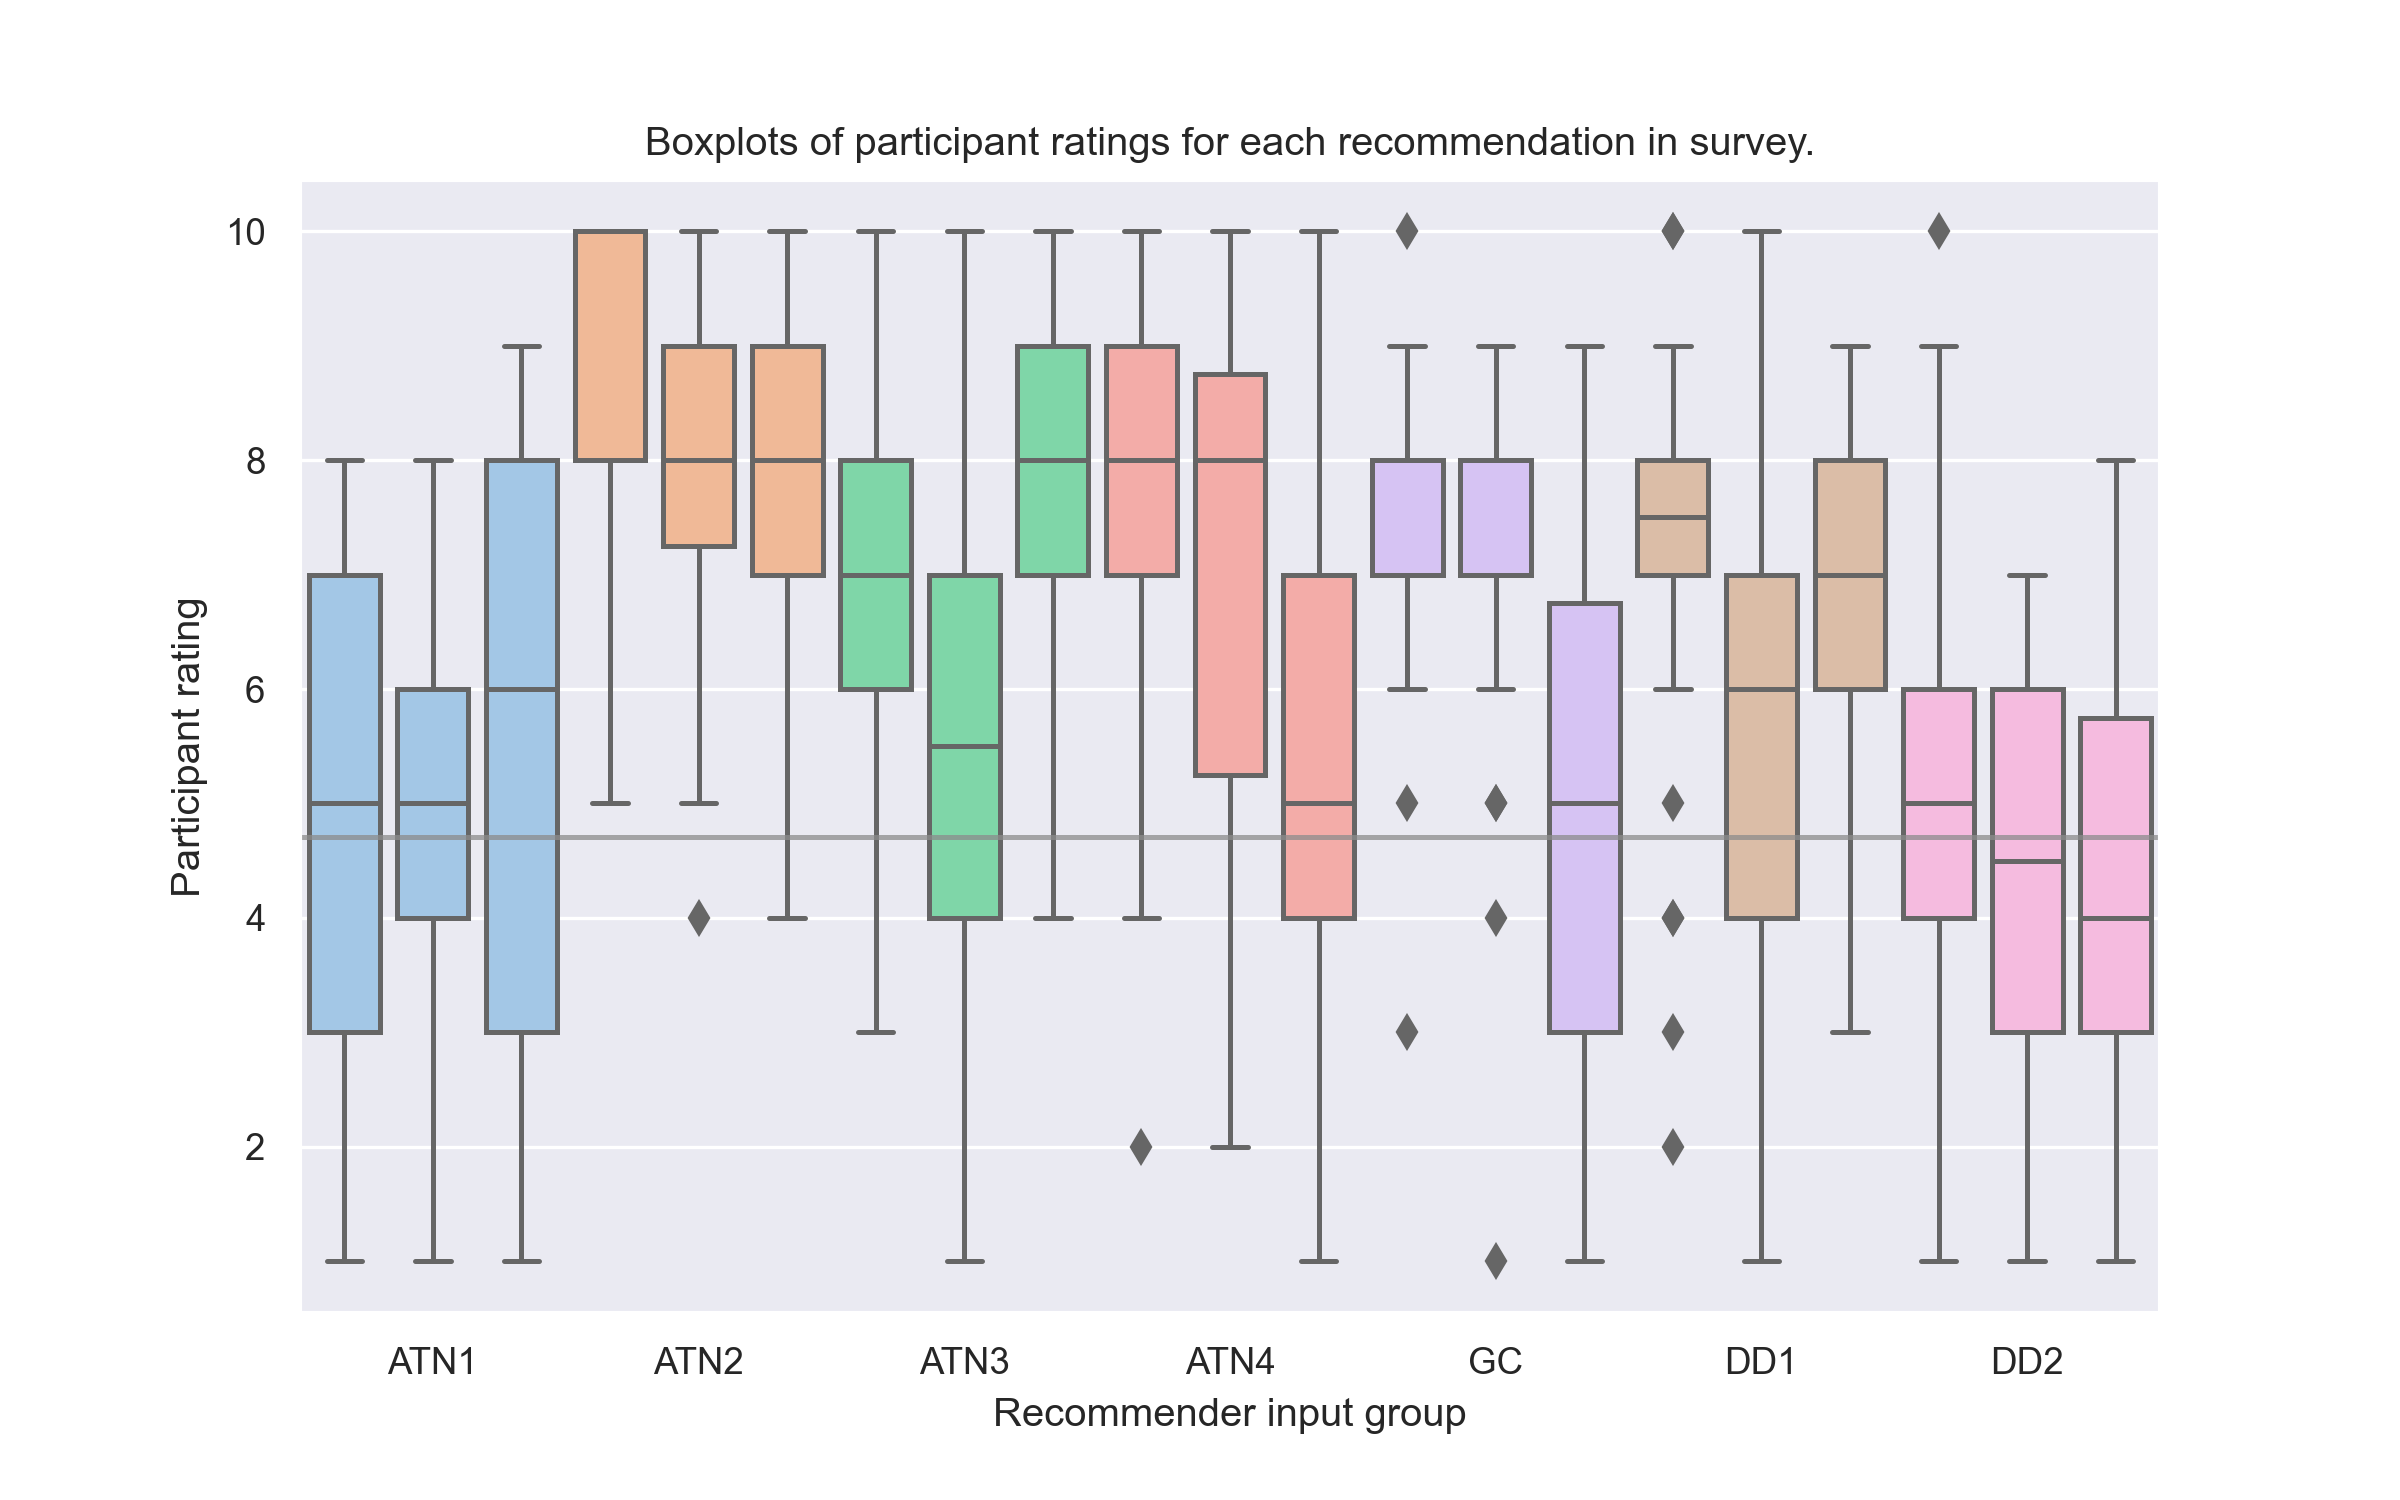
\includegraphics[width=0.8\textwidth]{graphics/all_recommendations}
        \caption{Boxplots of participant ratings for each recommendation, grouped by sample input. The grey line 
        indicates the mean baseline rating.}\label{fig:allrec}
    \end{figure}
\end{frame}


%------------------------------------------------
\section{Conclusions} 
%------------------------------------------------

\begin{frame}{Conclusions}
    
    \begin{itemize}
        \item Whisky recommender found to work
        \item More comprehensive evaluation needed
    \end{itemize}
    \begin{block}{Suggestions for Future Work}
        \begin{itemize}
            \item Front End UI
            \item Further comparisons of KE methods
            \item Work on whisky clustering
            \item Work with industry experts to more comprehensively evaluate and improve the agent
        \end{itemize}
    \end{block}

\end{frame}

\begin{frame}{Questions}
\textbf{Any Questions?}
\end{frame}

%----------------------------------------------------------------------------------------

\end{document}